\documentclass[12pt,a4paper]{article}
\usepackage[utf8]{inputenc}
\usepackage{amsmath}
\usepackage{amsfonts}
\usepackage{amssymb}
\usepackage{datetime}
\usepackage{float}
\usepackage{graphicx}
\usepackage{url}
\usepackage[separate-uncertainty=true]{siunitx}


\usepackage{pgfplots}
\usepackage{pgfplotstable}
\usepgfplotslibrary{groupplots}

\usepackage{booktabs} % for tables

\pgfplotsset{compat=newest}

\usepackage[labelfont=bf,textfont=md, font=footnotesize]{caption}

\usepackage[left=3.00cm, right=3.00cm, top=3.50cm, bottom=3.50cm]{geometry}

\usepackage{appendix}


\author{
    Ashot Matevosyan, Aram Matevosyan \\ Experiment performed \dayofweekname{18}{01}{2019} 18\textsuperscript{th} Januarty 2019
}
\title{Parameter estimation for the oscillating systems}



%\renewenvironment{abstract}
%{\par\noindent\textbf{\abstractname.}\ \ignorespaces}
%{\par\medskip}

\begin{document}
\maketitle
\begin{abstract}
\noindent 
	
	
\noindent Simple harmonic motion was investigated on a rotational oscillating system. Effect of dumping and forcing on motion of the system was examined and measurements were taken. Resonance in a oscillating system was investigated and quality factor of the dumping system was measured at different damping forces by three different methods.
Resonance curves were constructed at two different damping forces. Probabilistic model was built and system parameters were estimated from the resonance curves using Stan sampling platform. Quality factor of the oscillating system when "eddy brake" is turned off is estimated to be $Q = \num{71 \pm 1}$ and natural frequency $\omega_0 = \num{3.105 \pm 0.008}\, \si{\per\second}$.

\end{abstract}

\section{Introduction}
The aim of this experiment is to estimate parameters of the mechanical oscillating system by taking measurements.

In this experiment a torsion pendulum was used, motor for driving force with frequency control and "eddy brake"\cite{eddy-brake} for dumping.
Amplitude of the pendulum was measures versus number of complete oscillations and decay constant was measured. Resonance curves were found at two different damping forces. Quality factor was measures in three ways: by the decay constant, by resonance amplitude and by the resonance curve. For the analysis of the resonance curve Stan package\cite{stan} was used.

The necessary theory is summarized in the next section. Section \ref{section:methods} describes apparatus, illustrates method used and results of the experiment.Section \ref{section:stan} is dedicated to the parameter inference from the resonance curve. In section \ref{section:discuss} the results are discussed and the overall conclusions are provided in section \ref{section:conclusions}.
    
\section{Theoretical background}
	\subsection{The equation of motion}
	The equation of motion for an undamped torsional oscillator is
	\begin{equation} \label{eq:motion-undumped}
	I \ddot{\theta}+\tau \theta = 0
	\end{equation}
	where $I$ is moment of inertial of the oscillator, $\theta$ is the angular displacement from the equilibrium and the $\tau$ is the torsion constant. The general solution of this equation is
	\begin{equation} \label{eq:motion-undumped-sol}
	\theta = \theta_0 \cos(\omega_0 t + \phi) 
	\end{equation}
	where $\omega_0 = \sqrt{\cfrac{\tau}{I}}$ is the natural frequency of oscillation and $\phi$ is the initial phase.
	
	The system is damped if there is an opposing force proportional to $\dot{\theta}$. Now equation of motion \eqref{eq:motion-undumped} becomes
	\begin{equation} \label{eq:motion-dumped}
	I \ddot{\theta}+b\dot{\theta} + \tau \theta = 0
	\end{equation}
	where $b$ is constant. Finally, when sinusoidal driving force with angular frequency $\omega$ is applied, we get
	\begin{equation} \label{eq:motion-forced}
	I \ddot{\theta}+b\dot{\theta} + \tau \theta = A \cos(\omega t)
	\end{equation}
	The generalized form of these equations are
	\begin{equation} \label{eq:motion-general}
	\ddot{\theta}+2 \gamma \dot{\theta} + \omega_0^2 \theta = 0
	\end{equation}
	\begin{equation} \label{eq:motion-general-forced}
	\ddot{\theta}+2 \gamma \dot{\theta} + \omega_0^2 \theta = f \cos(\omega t)
	\end{equation}
	where $\omega_0 = \sqrt{\cfrac{\tau}{I}}$ is the\textit{natural frequency} of undamped oscillations, $2\gamma = \cfrac{b}{I}$ is a measure of damping and $f=\cfrac{A}{I}$ is a measure of driving amplitude.


	\subsection{Solution of generalized equation of motion}
	The general solution\cite{feynman-harmonic,feynman-transient} to equation \ref{eq:motion-general-forced} is the sum of the solution of equation \ref{eq:motion-general} (called \textit{transient response}) and a particular solution to eq. \ref{eq:motion-general-forced} (called \textit{steady state} or \textit{forced response}).
	
	The solution of eq. \ref{eq:motion-general} has three different solutions depending on the magnitude of damping. These difference cases are called \textit{underdamped}, \textit{overdamped} and \textit{critically damped}. The graphs for these cases for an oscillator which has been displaced from equilibrium and released from rest are shown in figures \ref{fig:underdamped}, \ref{fig:critical_over}, \ref{fig:critical_under} on the next page.
	\begin{figure}[ht]
		\centering
		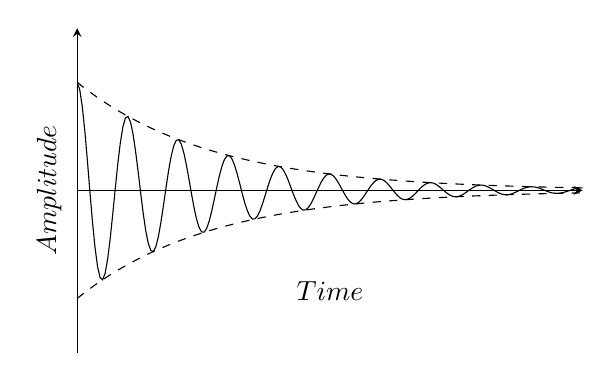
\begin{tikzpicture}
		\begin{axis}[
		height=5.7cm, width=8cm,
		domain=0:4*pi,
		xlabel= $Time$,
		ylabel=$Amplitude$,
		ymin=-1.5,ymax=1.5,
		%	axis lines=middle,
		axis x line=middle,
		axis y line=left,
		xtick=\empty,ytick=\empty,
		x label style={at={(axis description cs:0.5,+0.25)},anchor=north},
		]
		\addplot[black, samples=200]{exp(-x*0.3)* cos(deg(x*5))};	\addplot[black, dashed, samples=200]{exp(-x*0.3)};
		\addplot[black, dashed, samples=200]{-exp(-x*0.3)};
		\end{axis}
		\end{tikzpicture}
		\caption{Underdamped case, which has oscillatory motion.}
		\label{fig:underdamped}
	\end{figure}
	\begin{figure}[ht]
	\centering
	\begin{minipage}{.48\textwidth}
		\centering
		\begin{tikzpicture}
		\begin{axis}[
		domain=0:4*pi,
		xlabel= $Time$,
		ylabel=$Amplitude$,
		ymin=-1.5,ymax=1.5,
		%	axis lines=middle,
		axis x line=middle,
		axis y line=left,
		xtick=\empty,ytick=\empty,
		x label style={at={(axis description cs:0.5,+0.25)},anchor=north},
		]
		\addplot[black,dashed, samples=200]{exp(-x*2.5)*((2.5+2.37)*exp(+2.37*x) + (2.37-2.5)*exp(-2.37*x))/4.74};
		\addplot[black, samples=200]{exp(-0.8*x)*(1+0.8*x)};
		
		\end{axis}
		\end{tikzpicture}
		\caption{\textit{Critically damped} case, the dotted lines shows an \textit{overdamped} system with the same natural frequency.}
		\label{fig:critical_over}
	\end{minipage}%
	\hspace{.03\textwidth}
	\begin{minipage}{.48\textwidth}
		\centering
		\begin{tikzpicture}
		\begin{axis}[
		domain=0:4*pi,
		xlabel= $Time$,
		ylabel=$Amplitude$,
		ymin=-1.5,ymax=1.5,
		%	axis lines=middle,
		axis x line=middle,
		axis y line=left,
		x label style={at={(axis description cs:0.5,+0.25)},anchor=north},
		xtick=\empty,ytick=\empty,
		]
		\addplot[black,dashed, samples=200]{exp(-x*0.3)* cos(deg(x*2))};
		\addplot[black, samples=200]{exp(-0.3*x)*(1+0.3*x)};
		
		\end{axis}
		\end{tikzpicture}
		\caption{\textit{Critically damped} case, the dotted lines shows an \textit{underdamped} system with the same damping constant.}
		\label{fig:critical_under}
	\end{minipage}
	\end{figure}
	
	
	
	
	In particular, in the underdamped case, the transient response has the form
	\begin{equation}\label{eq:motion-transient}
	\theta = \theta_0 \, e^{-\gamma t} \cos(\omega_1 t)
	\end{equation}
	where $\omega_1=\sqrt{\omega_0^2-\gamma^2}$. $\gamma$ is called \textit{decay constant}.
	
	\textit{Quality factor} is a dimensionless parameter that describes how underdamped the oscillator is, how well it oscillates \cite{feynman-transient}. Quality factor Q is defined as
	\begin{equation}\label{eq:q-factor}
	Q=\cfrac{\omega_0}{2\gamma}
	\end{equation}
	For a \textit{good} oscillators $Q \gg 1$. 
	
	Forced response has the form
	\begin{equation}\label{eq:solution-forced}
	\theta(\omega)=X(\omega)\cos(\omega t - \phi(\omega))	
	\end{equation}
	where $\omega$ is the angular frequency of the driving force, and
	\begin{equation}\label{eq:solution-amplitude}
	X(\omega)=\frac{f}{\sqrt{(\omega_0^2-\omega^2)^2+(2 \gamma \omega)^2}}	
	\end{equation}
	\begin{equation}\label{eq:solution-phase}
	\tan \phi(\omega)=\frac{2\gamma \omega}{\omega_0^2-\omega^2}	
	\end{equation}
	$X(\omega)$ is the amplitude and $\phi(\omega)$ is the phase difference between driving force and oscillatory response. Graphs of these functions are shown on figure \ref{fig:amplitude-frequency} on the next page.
	\begin{figure}[ht]
		\centering
		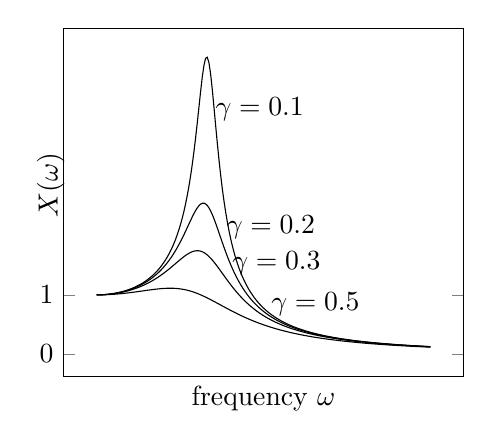
\begin{tikzpicture}[baseline]
		\begin{axis}[width=\textwidth*0.55,height=6cm,
		samples=200,domain=0:3,xlabel=frequency $\omega$, ylabel=$X(\omega)$,
		xtick=\empty,
		y label style={at={(axis description cs:-0.09,+0.55)},anchor=north},
		ytick={0,1}]
		\addplot[] {1/sqrt((1-x^2)^2+(2*x*0.1)^2)};
		\node at (axis cs:1.95,4.5) [anchor=north east] {$\gamma=0.1$};
		\addplot[] {1/sqrt((1-x^2)^2+(2*x*0.2)^2)};
		\node at (axis cs:2.05,2.5) [anchor=north east] {$\gamma=0.2$};
		\addplot[] {1/sqrt((1-x^2)^2+(2*x*0.3)^2)};
		\node at (axis cs:2.1,1.9) [anchor=north east] {$\gamma=0.3$};
		\addplot[] {1/sqrt((1-x^2)^2+(2*x*0.53)^2)};
		\node at (axis cs:2.45,1.2) [anchor=north east] {$\gamma=0.5$};
		\end{axis}
		\end{tikzpicture}%
		\hspace{0.25cm}
		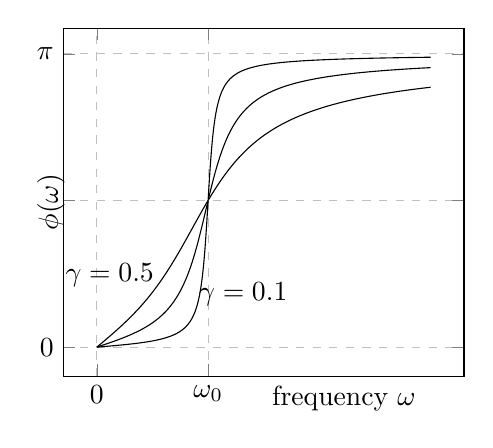
\begin{tikzpicture}[baseline]
		\begin{axis}[width=\textwidth*0.55,height=6cm,
		samples=200,domain=0:3,xlabel=frequency $\omega$, ylabel=$\phi(\omega)$,
		ytick={0, 1.57, 3.14},
		yticklabels={$0$, \empty,$\pi$},
		xtick={0,1},
		xticklabels={$0$, $\omega_0$},
		x label style={at={(axis description cs:+0.7,-0.0)},anchor=north},
		y label style={at={(axis description cs:-0.09,+0.5)},anchor=north},
		grid style=dashed,
		xmajorgrids=true,ymajorgrids=true]
		\addplot[domain=0:1] {rad(atan(2*x*0.05/(1-x^2)))};
		\addplot[domain=1+0.001:3] {pi+rad(atan(2*x*0.05/(1-x^2)))};
		\node at (axis cs:1.8,0.8) [anchor=north east] {$\gamma=0.1$};
		\addplot[domain=0:1] {rad(atan(2*x*0.2/(1-x^2)))};
		\addplot[domain=1+0.001:3] {pi+rad(atan(2*x*0.2/(1-x^2)))};
		\addplot[domain=0:1] {rad(atan(2*x*0.5/(1-x^2)))};
		\addplot[domain=1+0.001:3] {pi+rad(atan(2*x*0.5/(1-x^2)))};
		\node at (axis cs:0.6,1) [anchor=north east] {$\gamma=0.5$};
		\end{axis}
		\end{tikzpicture}
		\caption{Dependence of \textit{amplitude} (on the left) and \textit{phase difference} (on the right) from frequency of the driving force}
		\label{fig:amplitude-frequency}
	\end{figure}
	
	$X(\omega)$ gets its maximal value at
	
	\begin{align}
	\begin{split}
	\omega_{max} &= \sqrt{\omega_0^2-2\gamma^2} \\
	\text{and} \quad
	X_{max} \equiv X(\omega_{max}) &= \frac{f}{2\gamma\sqrt{\omega_0^2-\gamma^2}}
	\end{split}
	\label{eq:solution-omega-max}
	\end{align}
	
	Note that when $\gamma \ll \omega_0$, we can write
	\begin{align}
	\begin{split}
	X_{max} \approx \frac{f}{2\gamma\omega_0} &= \frac{f}{\omega_0^2} \cdot \frac{\omega_0}{2\gamma}\\
	&=X(0) \cdot Q
	\end{split}
	\label{eq:alt-q-factor}
	\end{align}
	The last step using definition of \textit{Quality factor} \eqref{eq:q-factor}, and $\cfrac{f}{\omega_0^2} = X(0)$ from the \linebreak equation \ref{eq:solution-amplitude}, i.e. amplitude when driving force has very big period.
	
\section{Methods and results}\label{section:methods}
   	\subsection{Apparatus}
   	Experiment was done on the oscillation system, consisting of:
   	\begin{itemize}
   		\item a bronze disc which undergoes rotational motion, the restoring couple, provided by a coiled spring, is linearly proportional to the angular displacement of the pendulum, which is measured by the scale around the disc.
		\item a motor, with frequency control. The pendulum can be driven sinusoidally by an arm connected to the motor. The frequency of the motor is controlled by the voltage across it. 
		\item two coils of wire which form an “eddy brake”, as a damping couple. Increasing the current in the eddy brake will increase the damping of the system.
	\end{itemize}
	Detailed diagram of the oscillating system is shown on the figure \ref{fig:system-diagram} above.
	\begin{figure}[t]
		\centering
		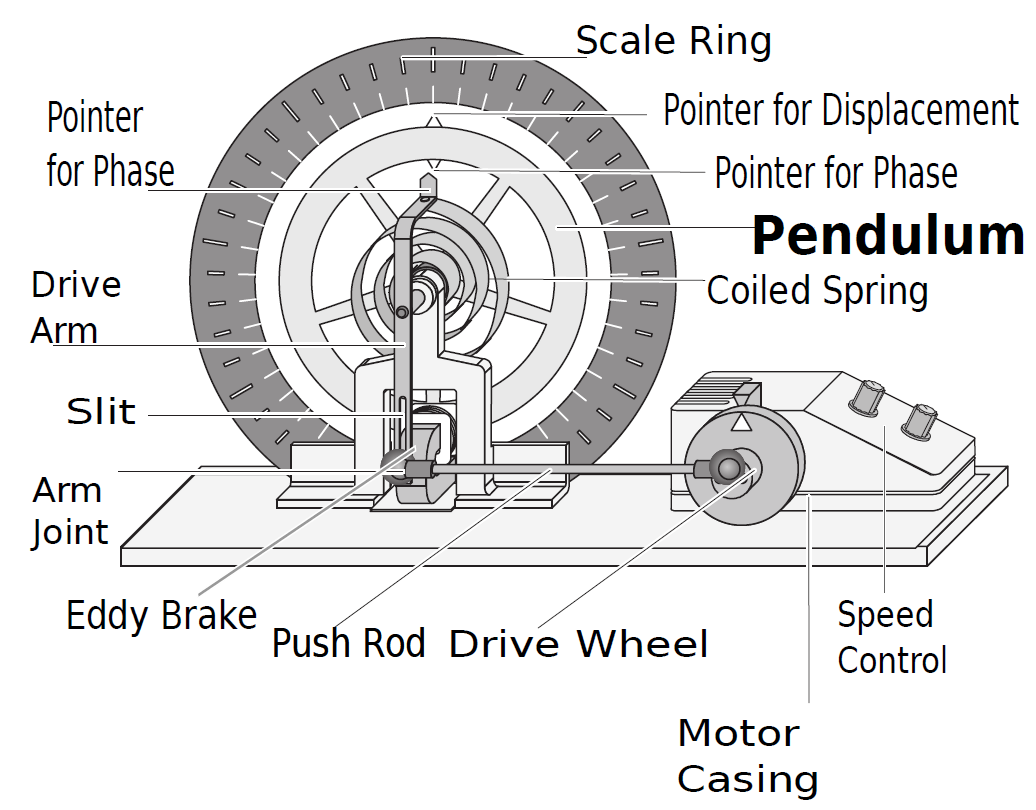
\includegraphics[width=0.6\linewidth]{images/pendulum_diagram.png}
		\caption{The diagram of the oscillating system in our experiment.}
		\label{fig:system-diagram}
	\end{figure}
	\subsection{Measurement of period of the pendulum}
	Four measurements of the time taken for ten complete periods of the pendulum were made. Results are shown on table \ref{table:measurement-period} and \ref{table:frequency}.
	\begin{table}[ht]
		\centering
		\begin{minipage}{.3\textwidth}
			\centering
			\begin{tabular}{ |c| } 
				\hline
				Time for 10 \\
				oscillations / \si{\second} \\
				\hline
				\num{20.35} \\
				\num{20.22} \\
				\num{20.10} \\
				\num{20.27} \\
				\hline
			\end{tabular}
			\caption{Measurements of 10 oscillations.}
			\label{table:measurement-period}
		\end{minipage}%
		\hspace{.1\textwidth}
		\begin{minipage}{.5\textwidth}
			\centering
			\begin{tabular}{ |c c| } 
				\hline
				mean & \num{20.24}\si{\second}  \\ 
				$\sigma$ & \num{0.10}\si{\second}  \\ 
				$\sigma_m$ & \num{0.05} \si{\second} \\ 
				\hline
				Period & \num[separate-uncertainty = true]{2.024 \pm 0.005} \si{\second}\\
				Frequency $\omega_1$ & \num[separate-uncertainty = true]{3.105 \pm 0.008} \si{\per\second}\\
				\hline
			\end{tabular}
			\caption{Period and angular frequency of the pendulum. "Eddy brake" is off.}
			\label{table:frequency}
		\end{minipage}
	\end{table}
	
	Even though "eddy brake" is off, i.e. current through it is zero, there is still damping force e.g. friction in the axle. But it is very small ($\gamma \ll \omega_0$) so we can assume $\omega_0 \approx\omega_1$ (see eq. \ref{eq:motion-transient})
\pagebreak
	\subsection{Measurement of amplitude}
	By the equation \ref{eq:motion-transient}, \textit{n-th successive oscillation} has an amplitude
	\begin{equation}\label{eq:n-th-amplitude}
	a_n = a_0 \, e^{-n \gamma T} 
	\end{equation}
	were $T=\cfrac{2 \pi}{\omega_1}$ is the period and $a_0$ is the initial amplitude. Taking logarithm on both sides, we get linear dependence from $n$:
	\begin{equation}\label{eq:ln-n-th-amplitude}
	\ln(a_n) = ln(a_0) - n \gamma T
	\end{equation}
	Experiment was done in two conditions: with no current through the eddy brake and with a braking current $I_b = 0.6 \,\si{\ampere}$, without driving force. In both cases the pendulum pendulum was released from rest at 10 on the scale. 
	
	To have more accurate measurements, the process was recorded by video camera, then amplitude was found from the replay in slow motion. Results are shown on figure \ref{fig:log-plot} below. 
	\begin{figure}[ht]
	\centering	
	\begin{tikzpicture}
	\begin{axis}[
	width=\linewidth,
	height=10cm,
	title={$ln(\text{amplitude})$ plotted as a function of the number of oscillations},
	xlabel={Number of oscillations, n},
	ylabel={$ln(\text{amplitude a\textsubscript{n} / arbitrary units})$ },
	xmajorgrids=true,ymajorgrids=true,
	grid style=dashed,
	]
	
	\addplot[
	color=blue,	only marks, mark=+,
	mark options={solid,scale=2,line width=0.5pt},
	error bars/.cd,
	y dir=both, y explicit,
	error bar style={line width=0.5pt,solid},
	error mark options={line width=0.7pt,mark size=3pt,rotate=90}
	]		
	table[x index = {0}, y index = {3}, y error plus index=4, y error minus index=5, col sep=comma]
	{data/transient_response_0.0A.csv};
	\addlegendentry{braking current = \SI{0.0}{\ampere}}
	
	\addplot [color=black,forget plot]
	table [col sep=comma, x index=0, 
	y={create col/linear regression={y=[index]3}}] 
	{data/transient_response_0.0A.csv};
	\xdef\slopeOne{\pgfplotstableregressiona}
	\xdef\interceptOne{\pgfplotstableregressionb}
	\node[] at (axis cs: 10,1.47){%
		$\pgfmathprintnumber{\slopeOne} \cdot x
		\pgfmathprintnumber[print sign]{\interceptOne}$};
	
	\addplot[color=orange, only marks, mark=+,
	mark options={solid,scale=2,line width=0.5pt},
	error bars/.cd,
	y dir=both, y explicit,
	error bar style={line width=0.5pt,solid},
	error mark options={line width=0.7pt,mark size=3pt,rotate=90}
	]		
	table[x index = {0}, y index = {3}, y error plus index=4, y error minus index=5, col sep=comma]
	{data/transient_response_0.6A.csv};
	\addlegendentry{braking current = \SI{0.6}{\ampere}}
	
	\addplot [color=black]
	table [col sep=comma, x index=0, 
	y={create col/linear regression={y=[index]3}}] 
	{data/transient_response_0.6A.csv};
	\xdef\slopeTwo{\pgfplotstableregressiona}
	\xdef\interceptTwo{\pgfplotstableregressionb}
	\node[] at (axis cs: 6,-0.53){%
		$\pgfmathprintnumber[precision=3]{\slopeTwo} \cdot x
		\pgfmathprintnumber[print sign]{\interceptTwo}$};
	
	\end{axis}
	\end{tikzpicture}
	\caption{Dependence of $\ln(\text{amplitude})$ from oscillation number $n$. Dependence is linear as we expect from equation \ref{eq:ln-n-th-amplitude}.}
	\label{fig:log-plot}
	\end{figure}

	\subsection{First estimation of quality factor} \label{section:qualiti-factor-estimation}
	From equation \ref{eq:ln-n-th-amplitude} a graph of $\ln(a_n)$ against $n$ should be a straight line with 
	\begin{equation}
	\text{slope of the line} =  -\gamma \, T = -\gamma \cfrac{2 \pi}{\omega_1}
	\end{equation}. 
	For low damping $\omega_1 \approx \omega_0$ so the slope is approximately $-\cfrac{\pi}{Q}$.
	By the statistical analysis of the data we got
	\begin{table}[H]\centering
	\begin{tabular}{c c} 
		\toprule
		slope [$I_b=0.0A]$ & \num{-0.044 \pm 0.001}\\
		slope [$I_b=0.6A]$ & \num{-0.80 \pm 0.03} \\
		\bottomrule
	\end{tabular}
	\end{table}
	And by assumption $\text{slope} \approx -\cfrac{\pi}{Q}$
	\begin{table}[H]\centering
		\begin{tabular}{c c} 
			\toprule
			Q [$I_b=0.0A$] & \num{71 \pm 1} \\
			Q [$I_b=0.6A$] & \num{3.9 \pm 0.1} \\
			\bottomrule
		\end{tabular}
	\end{table}
   	\subsection{Forced oscillations}
   	Now sinusoidal driving force is applied to the pendulum. General solution to the equation of motion \ref{eq:motion-general-forced} is superposition of transient response \eqref{eq:motion-transient} and forced response \eqref{eq:motion-forced}. As there is damping force, transient response vanishes over time and only forced response is viewed.
   	
   	Experiment was done with damping current of \num{0.3}\si{\ampere} and \num{0.6}\si{\ampere}. Frequency of the driving force was changed by the supply voltage and determined by taking time of 10 complete rotations of the drive wheel (see white mark on the wheel of the motor, figure \ref{fig:system-diagram}).
   	\subsection{Resonance curve}
   	Measurements was done by changing voltage of the driving motor, thus changing frequency of driving force. After some time only steady state solution (forced response) was seen. Amplitude was measured.
   	 
   	At first measurements was taken on the whole frequency range. Then more points were taken close to resonance frequency to define shape of resonance curve accurately.
   	
   	Results are shown on the figure \ref{fig:resonance-curve} and table \ref{table:resonance-results} on the next page.
   	
   	\begin{table}[H]
   		\centering
   		\begin{tabular}{c c c}
   			\toprule
   			& $X_{max}$ & $\omega_{max} $\\
   			\midrule
   			$I_b=\num{0.3}\si{\ampere}$ & \num{11.5 \pm 0.1} & \num{3.11 \pm 0.02} \si{\per\second}\\
   			$I_b=\num{0.6}\si{\ampere}$ & \num{3.3 \pm 0.1} & \num{3.05 \pm 0.05} \si{\per\second}\\
   			\bottomrule
   		\end{tabular}
   		\caption{Resonance frequency and the amplitude at resonance.}
   		\label{table:resonance-results}
   	\end{table}
      
   	\begin{figure}[ht]
   		\begin{tikzpicture}
   		\begin{axis}[
   		width=15cm,height=9cm,
   		title={Amplitude of forced oscillations as a function of angular frequency},
   		xlabel={Angular frequency / $s^{-1}$},
   		ylabel={Amplitude / arbitrary units},
   		xmajorgrids=true,ymajorgrids=true,
   		grid style=dashed,
   		]
   		
   		\addplot[smooth, solid,	color=blue,	mark=+,
   		mark options={solid,scale=2,line width=1.5pt}]		
   		table[x index = {3}, y index = {6}, col sep=comma]
   		{data/forced_oscillations_0.3A.csv};
   		\addlegendentry{braking current = \SI{0.3}{\ampere}}
   		\addplot [color=green,opacity=0.4, mark=*, mark size=5pt, forget plot] 
   		coordinates {(3.11,11.5)};
   		\draw [dashed,thick, color=black] (axis cs: -10,11.5) -| (axis cs: 3.11,-10);
   		
   		
   		\addplot[smooth, solid,	color=orange,	mark=+,
   		mark options={solid,scale=2,line width=1.5pt},
   		]		
   		table[x index = {3}, y index = {6}, col sep=comma]
   		{data/forced_oscillations_0.6A.csv};
   		\addlegendentry{braking current = \SI{0.6}{\ampere}}
   		\addplot [color=green,opacity=0.4, mark=*, mark size=5pt, forget plot] 
   		coordinates {(3.05,3.3)};
   		\draw [dashed,thick, color=black] (axis cs: -10,3.3) -| (axis cs: 3.05,-10);
   		
   		\end{axis}
   		\end{tikzpicture}
   		\caption{Resonance curve was found at different damping currents.}
   		\label{fig:resonance-curve}
   	\end{figure}
   
   \subsection{Second Estimation of quality factor} \label{section:qualiti-factor-estimation-2nd}
   Quality factor can be estimated using the equation \ref{eq:alt-q-factor}. But, at first, $X(0)$ need to be estimated.
   
   To measure the amplitude at $\omega=0$ the drive wheel was rotated  slowly by hand and the maximum displacement of the pendulum on either side of zero was read.
   
   Amplitude at $\omega = 0$ estimated to be $X(0) = \num{0.7 \pm 0.1}$. Thus
   \begin{table}[H]\centering
   	\begin{tabular}{c c} 
   		\toprule
   		$Q^{2nd}$ [$I_b=0.3A$] & \num{16 \pm 2} \\
   		$Q^{2nd}$ [$I_b=0.6A$] & \num{4.7 \pm 0.7} \\
   		\bottomrule
   	\end{tabular}
   \end{table}
  \section{Statistical analysis of resonance curve}\label{section:stan}
  \subsection{Model}
  From our experiment we have $(\omega_i, X_i)$ pairs for $i=1,...,n$, where $n$ is number of measurements. We can \textit{assume} that our measurements come from distribution
  \begin{equation}\label{eq:distribution}
  X_i \, \sim \,  
  \mathcal{P}(\,\, \cdot \,\, | \, \omega_i, \omega_0, X_0, \gamma) \equiv \mathcal{N}(X(\omega_i; \, \omega_0, X_0, \gamma),\,\sigma^{2})\ \quad 
  \text{   for   } i=1,...,n
  \end{equation}
  \begin{equation}\label{eq:solution-amplitude-new}
  X(\omega; \, \omega_0, X_0, \gamma) = \frac{X_0 \omega_0^2}{\sqrt{(\omega_0^2-\omega^2)^2+(2 \gamma \omega)^2}}
  \end{equation}
  
  where $\mathcal{N}(\mu, \sigma^2)$ is Normal distribution and $X(\omega; \, \omega_0, X_0, \gamma)$ (reparameterized version of eq. \ref{eq:solution-amplitude}) depends on parameters $\omega_0,\, \gamma$ and $X_0$ only. The latter one is amplitude at zero frequency.
  As precision of our measurements is 0.1, we take  $\sigma = 0.1$.
  Our task is to estimate parameters $\omega_0,\, \gamma$ and $X_0$ from the resonance curve $(\omega_i, X_i)_{1...n}$. More formally, find \textit{posterior distribution}
  
  \begin{equation}\label{eq:inference1}
  \omega_0, \, \gamma, \, X_0 \sim \mathcal{P}(\,\, \cdot \,\, | \, \omega_1...\omega_n, X_1...X_n)
  \end{equation}
  
  Unfortunately posterior distribution \ref{eq:inference1} is intractable. Therefore we do not have its analytical form to calculate moments of the parameters.
  
  However, without having explicit form of the posterior, we can make samples from that distribution.
  
  \subsection{Using \emph{Stan} sampling platform}
  Stan is a state-of-the-art platform for statistical modeling and high-performance statistical computation\cite{stan}. The Stan language is used to specify a (Bayesian) statistical model with an imperative program calculating the log probability density function. More about Stan in \url{mc-stan.org}.
  
  From the \textit{Bayes theorem}
  \begin{align}
  \begin{split}
  \mathcal{P}(\omega_0, \gamma,X_0\,|\,X_1...X_n, \omega_1...\omega_n) &=
  \cfrac{\mathcal{P}(X_1...X_n\,|\,\omega_0,\gamma,X_0,\omega_1...\omega_n) \cdot
  	\mathcal{P}(\omega_0,\gamma,X_0)
  }{\textit{margnal}} \\
&= \cfrac{\prod\limits_{i=1}^{n}\mathcal{P}(X_i\,|\,\omega_0,\gamma,X_0, \omega_i) \cdot
	\mathcal{P}(\omega_0,\gamma,X_0)
}{\textit{margnal}}
\end{split}
\label{eq:bayes-theorem}
  \end{align}
 
  
  
  where first term on the RHS is defined by our model (eq. \ref{eq:distribution})
  and second term is the \textit{prior distribution}, prior belief of parameters. We used \textit{Gamma distribution} as a prior. Therefore all term in the numerator of the equation \ref{eq:bayes-theorem} are defined, so we can do sampling.
  
  Stan uses MC-MC algorithm to draw samples from the distribution \ref{eq:bayes-theorem}. 
  
  \subsection{Results of sampling} \label{section:sampling-results}
  Mean and standard deviation of the samples were calculated and obtained values are shown in table \ref{table:resonance-infered-results} on the next page. Shape of the curve corresponding to inferred parameters is shown on figure \ref{fig:resonance-infered} to compare with experimental data.
  
  \begin{table}[ht]
  	\centering
  	\begin{tabular}{c c c}
  		\toprule
  		& $I_b=0.3\, \si{\ampere}$ & $I_b=0.6 \, \si{\ampere} $\\
  		\midrule
  		$\omega_0$ / \si{\per\second} & \num{3.10584 \pm 0.00012} & \num{3.1025 \pm 0.0013} \\
  		$\gamma$ / \si{\per\second} & \num{0.09059 \pm 0.00016} & \num{0.3363 \pm 0.0018} \\
  		$X_0 \equiv X(0)$ & \num{0.6675 \pm 0.0010} & \num{0.708 \pm 0.003} \\
  		$Q^{3th}$ / \si{\per\second} & \num{17.14 \pm 0.03} & \num{4.61 \pm 0.02} \\
  		\bottomrule
  	\end{tabular}
  	\caption{Resonance frequency and the amplitude at resonance.}
  	\label{table:resonance-infered-results}
  \end{table}
  
  \begin{figure}
  	\begin{tikzpicture}
  	\begin{groupplot}[group style={group size=2 by 1}]
  	\nextgroupplot[
  	ylabel={Amplitude / arbitrary units},
  	xmajorgrids=true,ymajorgrids=true,
  	xminorgrids=true,yminorgrids=true,
  	grid style=dashed]
  	\addplot[color=blue, mark=+,only marks, 
  	mark options={solid,scale=2,line width=1.5pt}]		
  	table[x index = {3}, y index = {6}, col sep=comma]
  	{data/forced_oscillations_0.3A.csv};
  	\addlegendentry{$I_b$ = \SI{0.3}{\ampere}}
  	\addplot[domain=0:6, samples=200] {0.6675 * 3.106^2/sqrt((3.106^2-x^2)^2+(2*x*0.0906)^2)};
  	
  	
  	\nextgroupplot[xlabel={Angular frequency / $s^{-1}$},
  	xmajorgrids=true,ymajorgrids=true,
  	xminorgrids=true,yminorgrids=true,
  	grid style=dashed,
  	x label style={at={(axis description cs:-0.1,-0.08)},anchor=north},
  	legend pos=north west
  	]
  	\addplot[color=orange,	mark=+, only marks,
  	mark options={solid,scale=2,line width=1.5pt},
  	]		
  	table[x index = {3}, y index = {6}, col sep=comma]{data/forced_oscillations_0.6A.csv};
  	\addlegendentry{$I_b$ = \SI{0.6}{\ampere}}
  	\addplot[domain=0:5, samples=200] {0.708 * 3.1025^2/sqrt((3.1025^2-x^2)^2+(2*x*0.336)^2)};
  	\end{groupplot}
  	\end{tikzpicture}
  	\caption{Form of the resonance curve using parameters found by inference.}
  	\label{fig:resonance-infered}
  \end{figure}

\section{Discussion}\label{section:discuss}
	\subsection{Consistence with theory}
	From the figure \ref{fig:log-plot} we see that points lie quite well on the line, which was predicted by the equation \ref{eq:ln-n-th-amplitude}. Also when we increase damping force we get lower quality factor as expected from equation \ref{eq:q-factor}.
	
	In the case of forced oscillations, our resonance curves shown on figure \ref{fig:resonance-curve} have the same shape as on figure \ref{fig:amplitude-frequency} derived from theory.
	
	In case of lower damping we have higher resonance amplitude, which also consistent with equation \ref{eq:solution-amplitude} (also visualized on figure \ref{fig:amplitude-frequency} ).
	However at lower damping we should have higher \textit{resonance frequency} which follows from equation \ref{eq:solution-omega-max}, but from the results of table \ref{table:resonance-results} it is not obvious.
	
	\subsection{Three estimations of quality factor}
	We estimated quality factor by three different ways at same damping:
	\begin{itemize}
		\item $Q=\num{3.9 \pm 0.1}$ -- transient response method, section \ref{section:qualiti-factor-estimation}
		\item $Q=\num{4.7 \pm 0.7}$ -- forced response method, section \ref{section:qualiti-factor-estimation-2nd}
		\item $Q=\num{4.61 \pm 0.02}$ -- resonance curve method, section \ref{section:sampling-results}
	\end{itemize}
	Second and third values consistent with each other. Note that big error of the second estimation comes from measurement of $X(0)$ with high uncertainty.
	However, first and third values are very different, there could have been systematic error in picking braking current.
	
	\subsection{Improvements to the experiment}
	At high damping, e.g. $I_b = 0.6 \si{\ampere}$ approximation $\omega_1 = \sqrt{\omega_0^2-\gamma^2} \approx \omega_0$ is not accurate anymore. On the other hand we can easily measure frequency $\omega_1$. Thus we will have better estimation of quality factor.
	
	We can construct better resonance curve (fig. \ref{fig:resonance-curve}) by simply taking more measurements. Also we can calculate quality factor from the bandwidth of the resonance curve\cite{feynman-resonance}, and compare it with previous methods.
	
\section{Conclusions}\label{section:conclusions}
	We have shown that our measurements are consistent with theory, e.g. exponentially decaying amplitude, shape of the resonance curve.
	
	We provided different methods of analysis of the measurements and inference of system parameters such as \emph{natural frequency}, \emph{decaying factor}, etc.

	Probabilistic method of inferring system parameters described in section \ref{section:stan} resulted in estimations with high precision. So we can conclude that ~10 points of the resonance curve contain all the information of the system.
	
	
\pagebreak
\begin{thebibliography}{9}
    \bibitem{eddy-brake} Cadwell, L. H. (1996). \emph{Magnetic damping: Analysis of an eddy current brake using an airtrack}. American Journal of Physics, 64(7), 917–923. doi:10.1119/1.18122 
    
    \bibitem{feynman-harmonic} \emph{The Feynman lectures on physics}, Vol. I: Chapter 21: The Harmonic Oscillator
    
   \bibitem{feynman-transient} \emph{The Feynman lectures on physics}, Vol. I: Chapter 24: Transients
   
       
   \bibitem{feynman-resonance} \emph{The Feynman lectures on physics}, Vol. I: Chapter 23: Resonance
    
    \bibitem{stan} Bob Carpenter, Andrew Gelman, Matthew D. Hoffman, Daniel Lee, Ben Goodrich, Michael Betancourt, Marcus Brubaker, Jiqiang Guo, Peter Li, and Allen Riddell. 2017. \emph{Stan: A probabilistic programming language}. Journal of Statistical Software 76(1). DOI 10.18637/jss.v076.i01
    
    
\end{thebibliography}



\end{document}